\documentclass[tikz,dvipdfmx]{standalone}

\usepackage{amsmath, amssymb, amsthm, mathrsfs, amsfonts, dsfont}
\usepackage{mathtools}

\usetikzlibrary{
  decorations.pathreplacing,
  decorations.pathmorphing,
  decorations.markings,
  shapes.geometric,
  calc,
  arrows.meta,
  positioning,
  fit,
  backgrounds,
  patterns,
  3d,
}

\definecolor{cA}{HTML}{0072BD}
\definecolor{cB}{HTML}{EDB120}
\definecolor{cC}{HTML}{77AC30}
\definecolor{cD}{HTML}{D95319}

\begin{document}

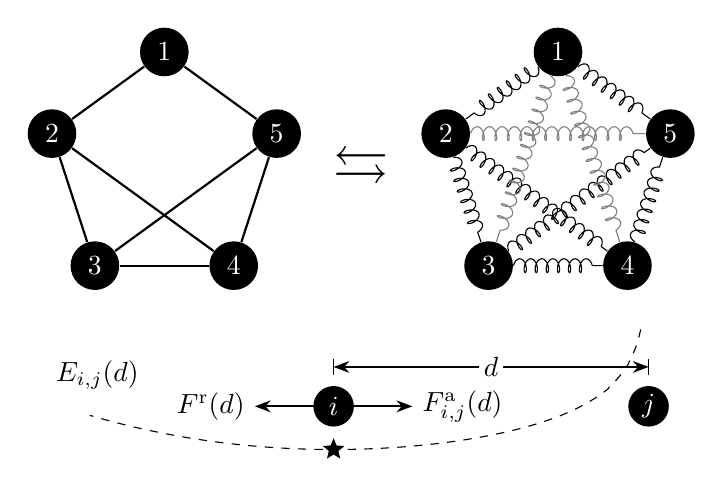
\begin{tikzpicture}
  \begin{scope}[xshift=-2.5cm]
    \foreach \i in {1,...,5}{
        \node[circle, fill=black, text=white,minimum size=0.5cm] (a\i) at ({90+72*(\i-1)}:1.5) {\i};
      }
    \foreach \i/\j in {1/2,1/5,2/3,2/4,3/4,3/5,4/5}{
        \draw[thick] (a\i) -- (a\j);
      }
  \end{scope}
  \begin{scope}[xshift=+2.5cm]
    \foreach \i in {1,...,5}{
        \node[circle, fill=black, text=white, minimum size=0.5cm] (a\i) at ({90+72*(\i-1)}:1.5) {\i};
      }
    \foreach \i/\j in {1/2,1/5,2/3,2/4,3/4,3/5,4/5}{
        \draw[decorate, decoration={coil, segment length=4}] (a\i) -- (a\j);
      }
    \foreach \i/\j in {1/3,1/4,2/5}{
        \draw[decorate, decoration={coil, segment length=4.5},gray] (a\i) -- (a\j);
      }
  \end{scope}

  \node[scale=2] at (0,0) {$\leftrightarrows$};

  \begin{scope}[xshift=-0.35cm, yshift=-3cm]
    \def\d{4}
    \def\r{0.25}
    \def\u{1.0}
    \coordinate (M1) at (0,0);
    \coordinate (M2) at (\d,0);

    \draw[fill=black] (M1) circle (\r) node[white] {$i$};
    \draw[fill=black] (M2) circle (\r) node[white] {$j$};

    \draw (0,+1.6*\r) -- (0,+2.4*\r);
    \draw (\d,+1.6*\r) -- (\d,+2.4*\r);
    \draw[{Stealth[length=2mm]}-{Stealth[length=2mm]}] ($(M1)+(90:2*\r)$) -- ($(M2)+(90:2*\r)$)
    node[midway,circle,fill=white,inner sep=0] {$d$};

    \draw[-{Stealth[length=2mm]},thick,line cap=round] (+\r,0) -- (+\u,0) node[right] {$F_{i,j}^\mathrm{a}(d)$};
    \draw[-{Stealth[length=2mm]},thick,line cap=round] (-\r,0) -- (-\u,0) node[left] {$F^\mathrm{r}(d)$};

    \draw[dashed,domain=3.9:-3.1,samples=1000,smooth,variable=\x] plot(\x,{-0.7+(pow((\d-\x)/\d,3)/3-ln((\d-\x)/\d))/2.2});
    \node [star,
      minimum size=0.25cm,
      star point ratio=2.25,
      inner sep=0pt,
      draw, fill=black]
    at (0,{-0.7+(1/3)/2.2}) {};

    \node at (-3,0.4) {$E_{i,j}(d)$};
  \end{scope}
\end{tikzpicture}

\end{document}